\documentclass[11pt, a4paper, reqno]{scrartcl}

\usepackage[utf8]{inputenc}
\usepackage{a4wide}
\usepackage{libertine}
\usepackage{graphicx}
\usepackage{listings}
\usepackage{xcolor}
\usepackage{float}
\usepackage{amsmath}
\usepackage{microtype}

% for latex output of pandas
\usepackage{booktabs}

\begin{document}
    \title{Exercise No. 7}
    \author{David Bubeck, Pascal Becht, Patrick Nisbl\`e}
    \maketitle
    
    \lstset{
        language=Python,
        backgroundcolor=\color{gray!5},
        numbers=left,
        captionpos=t,
        breaklines=true,
        frame=l,
        xleftmargin=\parindent,
        basicstyle=\footnotesize\sffamily,
        keywordstyle=\bfseries\color{green!40!black},
        commentstyle=\itshape\color{purple!40!black},
        identifierstyle=\color{blue!60!black},
        stringstyle=\color{orange}
    }

	 \section{Population dynamics}
		 \subsection{Dimension Analysis}
		 
		 In this exercise we should analyze the following equation for population dynamics,
		 \begin{equation}
		 \frac{dN}{dt} = r N \bigg(1 - \frac{N}{K} \bigg) - \frac{B N^2}{A^2 + N^2}\, ,
		 \end{equation}
		 with the parameters $r, k, A, B > 0$.
		 To bring the equation in dimensionless form it is useful to think about the dimensions of each parameter. 
		 
		 First look at the right part of the right hand side of the equation. 
		 From the denominator we see that the dimension of $A$ must be equal to this of $N$.
		 Next it is clear that $B$ must have the same dimension that the left hand side, to achieve the corresponding dimension for the whole right term. 
		 For the left term of the right hand side, it is clear that $r$ is a rate and therefore has dimension $1/time$. The fraction in the brackets makes clear, that $K$ has the same dimension than $N$, and so we have determined all dimensions and everything is consistent.
		 
		 In the tabular below the dimensions are listed to give a review.
		 \vspace{5pt}
		 \begin{center}
		 	\begin{tabular}{ll}
		 		\hline
		 		Parameter&Dimension\\
		 		\hline
		 		N&whatever the population is\\
		 		A&same than N\\
		 		B&N over time\\
		 		r&one over time\\
		 		K&same than N\\
		 		\hline
		 	\end{tabular}
		 \end{center}
		 \vspace{10pt}
		 
		 The next step is to make the equation dimensionless. 
		 We start with the hints given on the exercise sheet, so that 
		 \[
		 n = \frac{N}{A}\]
		 Further we choose 
		 \[
		 k = \frac{K}{A}\, .\]
		 
		 Inserting this into the above equation we yield
		 \begin{equation}
		 \frac{dn}{dt} = r n \bigg(1 - \frac{n}{k}\bigg) - \frac{B}{A} \cdot \frac{n^2}{1 + n^2}
		 \end{equation}
		 Next we want do have a dimensionless time $\tau$. 
		 Because we want a $\tau$ independent of $r$, we choose 
		 \[
		 \tau = \frac{B}{A} t\, , \]
		 Inserting this we become
		 \begin{equation}
		 \frac{dn}{d \tau} = \frac{A}{B} \frac{dn}{dt} = r \frac{A}{B} n \bigg(1 - \frac{n}{k} \bigg) - \frac{n^2}{1 + n^2}
		 \end{equation}
		 \begin{equation}
		 \Leftrightarrow \quad \frac{dn}{d \tau} = R n \bigg(1 - \frac{n}{k} \bigg) - \frac{n^2}{1 + n^2}\, ,
		 \end{equation}
		 with 
		 \[
		 R = r \frac{A}{B}\, .\]
		 
		 In the end we achieved a dimensionless representation of the above equation, with only owo remaining free parameters, which are $R$ and $k$.
		 \\
		 
	\subsection{Fix Point Analysis}
		 In the second part of the exercise we are analyzing the fix points of the dimensionless equation.
		 The fix points are defined as the roots of the right hand side
		 \[
		 f(n) = R n \bigg(1 - \frac{n}{k} \bigg) - \frac{n^2}{1 + n^2} \]
		 First we set $k = 7.5$ as told in the exercise sheet.
		 The first trivial fix point is $n^{\ast} = 0$.
		 To determine the other fix points we reshape the equation for $f(n)$, which then is
		 \begin{equation}
		 f(n) = R \bigg[1 + n^2 \bigg(1 - \frac{1}{7.5} \bigg) - \frac{n^3}{7.5} \bigg] - n = 0
		 \label{eq: findroot}
		 \end{equation}
		 This cubic function can be plotted with varying $R$ to determine the roots roughly and see how many roots there are.
		 We can find two real roots for $R = 0.6$, which is shown in figure \ref{fig: 1}.
		 The roots were searched with the Mathematica function 'FindRoot' and the results are, 
		 \[
		 n^{\ast}_{11} = 1.33333\]
		 \[
		 n^{\ast}_{12} = 4.36556\, .\]
		 Taking other values for $R$, only one root can be found. 
		 \begin{figure}[H]
		 	\centering
		 	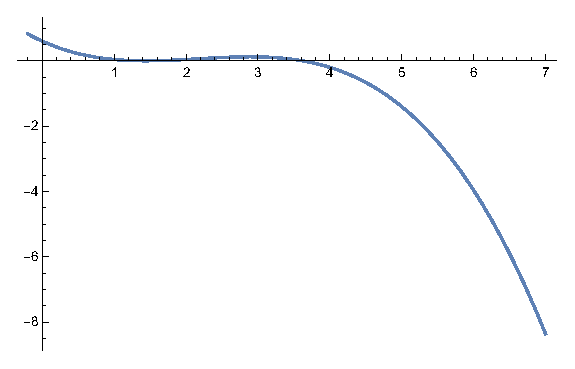
\includegraphics[]{CompPhys_6-2_gr1.eps}
		 	\caption{Plot of equation \eqref{eq: findroot} for $R = 0.6$.}
		 	\label{fig: 1}
		 \end{figure}
	 
	 	 Because equation \eqref{eq: findroot} is cubic, there must be up to three roots for some combination of parameters.
	 	 \[n^{\ast}_{11} = 1.38197\]
	 	 \[n^{\ast}_{12} = 3.61803\]
	 	 
	 	 With $n^{\ast}_{11}$ being a Saddle point with $y=0$.
	 	 
	 	 We also tried applying other parameters to get 3 roots:
	 	 
	 	 \begin{figure}[H]
	 	 	\centering
	 	 	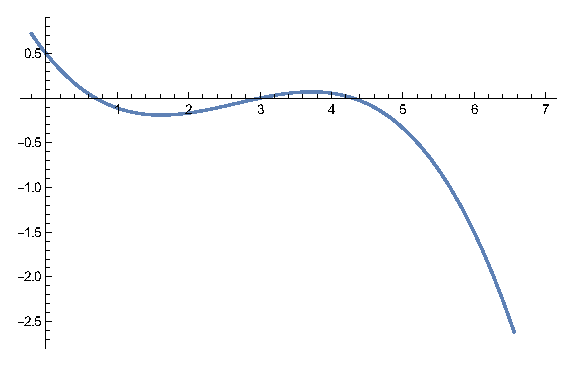
\includegraphics[]{CompPhys_6-2_gr3.eps}
	 	 	\caption{Plot of equation \eqref{eq: findroot} for $R = 0.5$ and $k=9$.}
	 	 	\label{fig: 2}
	 	 \end{figure}
	 	 \[n^{\ast}_{21} = 0.697224\]
	 	 \[n^{\ast}_{22} = 3.0\]
	 	 \[n^{\ast}_{23} = 4.30278\]
	 	 \begin{figure}[H]
	 	 	\centering
	 	 	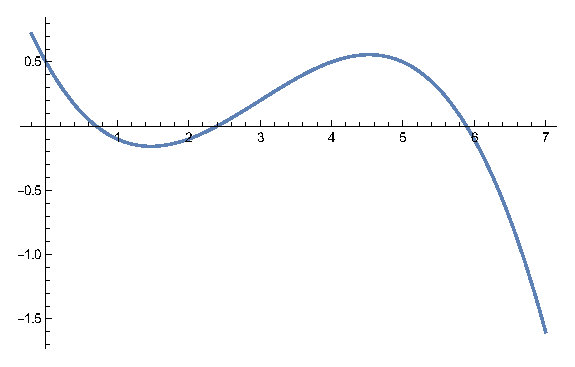
\includegraphics[]{CompPhys_6-2_gr2.eps}
	 	 	\caption{Plot of equation \eqref{eq: findroot} for $R = 0.5$ and $k=10$.}
	 	 	\label{fig: 3}
	 	 \end{figure}
	 	 \[n^{\ast}_{31} = 0.707598\]
  		 \[n^{\ast}_{32} = 2.3973\]
		 \[n^{\ast}_{33} = 5.89511\]
		 
		 Now we can analyze if the fix points are stable or unstable. 
		 The criteria for a stable fix point is that the derivative in this point is smaller than zero and vice versa for unstable fix points.
		 This means simply that if the slope of the plotted graph is negative in the fix point its stable and if the slope is positive its unstable. 
		 
		 Applying this on the found values we get 
		 \[n^{\ast}_{12},n^{\ast}_{21},n^{\ast}_{23},n^{\ast}_{31},n^{\ast}_{33}  \Rightarrow stable \]
		 \[n^{\ast}_{22}, n^{\ast}_{32} \Rightarrow unstable\, .\]
		 \[n^{\ast}_{11} \Rightarrow uncertain\]
 	 	 
	 	 
	 	
\end{document}